\documentclass{book}

\usepackage{amsmath}
\usepackage{amssymb}
\usepackage{xfrac}
\usepackage{todonotes}
\usepackage{array}
\usepackage{float}

\addtolength{\oddsidemargin}{-.875in}
\addtolength{\evensidemargin}{-.875in}
\addtolength{\textwidth}{1.75in}
\addtolength{\topmargin}{-.875in}
\addtolength{\textheight}{1.75in}

\newcolumntype{M}[1]{>{\centering\arraybackslash}m{#1}}

\title{Bioengineering Imaging Track Qualifying Exam Study Book}
\author{Markus Foote and Blake Zimmerman}

\begin{document}
	\maketitle
	\tableofcontents
		\part{Essential Mathematics}
			\chapter{Fourier Theory} The {\em Fourier transform} is analogous to the separation of white light into a rainbow by a prism. This mathematical operator has many useful applications in imaging. We define the Fourier transform of a function $g$ as
\begin{equation}
G(f)=\mathcal{F}\left\{g(t)\right\} = \int_{-\infty}^{\infty} g(t) e^{-i2\pi ft}\, dt \;.
\end{equation}
We define the inverse of this operation as
\begin{equation}
g(t)=\mathcal{F}^{-1}\left\{G(f)\right\} = \frac{1}{2\pi}\int_{-\infty}^{\infty} G(f) e^{i2\pi ft}\, df \;.
\end{equation}
These definitions are not unique, especially in the handling of the normalizing factors; it is also common to see a $\sfrac{1}{\sqrt{2\pi}}$ coefficient in \emph{both} forward and inverse operations.

The Fourier transform can also be considered as a linear operation (which it is), in terms of vectors and matrices.

\todo{examples here}

The Fourier transform has many useful properties, some of which are listed in Table \ref{tab:fourierProperties} .

\begin{table}
	\caption{\label{tab:fourierProperties} Fourier Transform Properties}
	{\renewcommand{\arraystretch}{2}%
	\begin{tabular}{|c|M{6.5cm}|p{4.5cm}|}
		\hline
		{\textbf{Name}} & {\textbf{Formula}} &{\textbf{Notes}} \\
		\hline\hline
		Linearity& $\mathcal{F}\left\{\alpha\, g_1(t) + \beta\, g_2(t)\right\} = \alpha\, G_1(f) + \beta\, G_2(f)$ & $\alpha$, $\beta$ may be complex.\\
		\hline
		Scaling & $\mathcal{F}\left\{g(\alpha t) \right\} = \frac{1}{|\alpha|}G(\frac{f}{\alpha})$& $\alpha > 1$ compresses $g$ in time $\to$ expands in frequency\\
		\hline
		Duality & $\mathcal{F}\left\{G(t)\right\}=g(-f)$& \\
		\hline
		Shifting & $\mathcal{F}\left\{g(t-\tau)\right\}= G(f) e^{-i2\pi f\tau}$  & \\
		\hline
		Convolution & 
		{$\begin{aligned}%
		\mathcal{F}\left\{ g_1(t) \circledast g_2(t)\right\} & =  G_1(f) \cdot G_2(f) \\ \mathcal{F}\left\{ g_1(t) \cdot g_2(t)\right\} & = G_1(f) \circledast G_2(f)
		\end{aligned}$}&\\
		\hline
	\end{tabular}}
	
\end{table}


			\chapter{Convolution} 
Convolution can be interpreted in two main ways:
\begin{description}
	\item[Repetition] of an action on a single point to the entire input
	\item[Superposition] of replicas of a function weighted by another function
\end{description}

Convolution has important mathematical properties:
\begin{enumerate}
	\item Commutative Property $f \circledast g = g \circledast f$
	\item Replicating Property $f(t) \circledast \delta(t) = f(t)$
	\item Shifting Property $ f(t) \circledast \delta(t-\tau) = f(t-\tau)$	
\end{enumerate}


			\chapter{Signal Processing} \subsection{LTI Systems Definitions}
Systems theory is largely based on the assumption that a system being inspected is \emph{Linear and Time or Translation-Invariant}, or LTI. This property of a system is satisfied by these two requirements: 
\begin{enumerate}
	\item Linear: a scaled input produces a same-scaled output.
	\item Time/Translation-Invariant: a delayed (or earlier) input produces a delayed (or earlier) output which is otherwise identical to the output from the non-delayed input.
\end{enumerate}
The LTI system property makes the input-output relationship more predictable. However, this condition is fairly easy to break; for example, the magnitude-calculation "system" is \emph{not} something \todo{linear/time invariant}: $h(x+iy) = \sqrt{x^2 + y^2} \neq  h(\alpha ...)$

\subsection{System Response}
For an LTI system, the output is well-defined from the input, $x$ and the system's impulse response, $h(\delta(t))$. The output, $y$, is easily calculated as $h(t)\circledast x(t)$. Using the convolution theorem of the Fourier transform, this output can also be calculated in the frequency domain: $Y(f) = H(f)\cdot X(f)$ and the output in time is easily calculated through an inverse Fourier transform. This approach is typically employed when the steady-state output of a system is desired. The Fourier transform-based approach is advantageous because it is less computationally-intensive than a convolution. However, the convolution-based approach is necessary in the following cases:
\begin{enumerate}
	\item Solution for output before the system reaches steady-state is required.
	\item Real-time output is required.
\end{enumerate}
Additionally, the convolution-based approach is computationally advantageous when the kernel is relatively short.
			\chapter{Discrete Representations}
				\section{Derivatives}
					\subsection{Gradient}
					\subsection{Laplacian}
					%\subsection{Inversion Techniques / Integration}
				\section{Fourier Transforms}
				\section{Convolution}
				
		\part{MRI}
			\chapter{Essential Physics}
				\section{Nuclear Magnetic Resonance}
				\section{Spatial Encoding}
				\section{Slice Selection}
				\section{Field of View}
				\section{Sampling Patterns}
				\section{Image Formation and Image Quality Measures}
					\subsection{Resolution}
					\subsection{Contrast}
					\subsection{Common Reconstruction Artifacts}
					\subsection{Partial Volume Effects}
			\chapter{Fourier Transform}
				\section{Fourier Transform Properties}
				\section{Image Reconstruction}
			\chapter{Advanced MR Techniques}
				\section{Fat Suppression}
				\section{Diffusion Weighted Imaging and DTI}
				\section{EPI}
				\section{Temperature Sensitive Imaging}
				\section{BOLD}
		
		\part{CT}
			\chapter{CT Physics}
				\section{X-Ray Physics}
					\subsection{History (Do we really need this)}
Projection Radiography was pioneered by R\"oentgen in 1895. 

\subsection{X-Ray Creation}
X-Rays are created when kinetic energy of an electron is converted into electromagnetic radiation, usually via interaction with a target material, called the anode. These electrons are generated from a heating element cathode and accelerated toward the target anode via the voltage between the cathode and anode. The kinetic energy of these electrons is proportional to the electrical charge and potential difference between the cathode and anode. Figure ~\ref{fig:xrtube} shows a labeled X-ray tube to depict the general layout. An important note that the anode is a spinning disk to help dissipate the generated heat. The most common material used for the cathode and anode is tungsten. 

\begin{figure}[H]
	\centerline{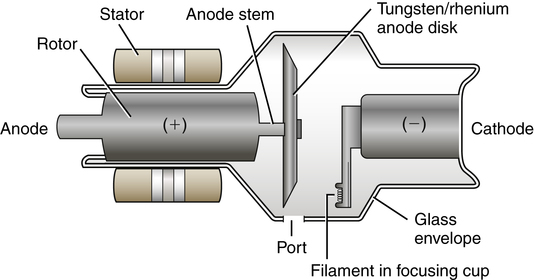
\includegraphics[width=.6\columnwidth,height=4cm]
		{images/xray_tube.jpg}}
	\caption{\label{fig:xrtube} Image of a typical X-Ray tube. The apparatus is enclosed in a vacuum to limit the electrons interactions with air particulates. }
\end{figure}

When the electrons released from the cathode interact with anode material, there is always release of radiation, known as Bremsstrahlung radiation. Depending on the incident angle of the electron and the distance to the atom that it interacts with, varying levels of radiation are given off. This radiation is generated because the incident electron is slowed by the target atomic nucleus, reducing kinetic energy of the incident electron, resulting in the release of radiation. An incident electron can also collide with a target electron, and if the energy exceeds that of the target electron's binding energy, that target electron is ejected. As there is now a vacancy in one of the atoms electron shells, an electron from a lower energy shell will immediately transition to fill it, giving off what is known as characteristic radiation.  Figure \ref{fig:brem} shows a filtered radiation spectrum including the characteristic radiation from an example target material. 


\begin{figure}[H]
	\centerline{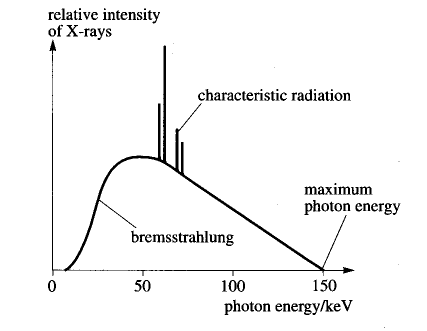
\includegraphics[width=.6\columnwidth,height=4cm] 
		{images/brem.png}}
	\caption{\label{fig:brem} Example radiation spectrum including characteristic radiation. }
\end{figure}
				\section{Sampling Theorem}
				\section{Image Formation and Image Quality}
					\subsection{Resolution}
					\subsection{Contrast}
			\chapter{Radon Transform}
			\chapter{Reconstruction Techniques}
				\section{Central Slice Theorem}
				\section{Projection}
				\section{Backprojection}
			\chapter{Practical Considerations}
				\section{Beam Hardening}
				\section{Partial Volume Effects}
				\section{Common Reconstruction Artifacts}
			\chapter{Advanced }
			
		%\part{Ultrasound}
		
		
		\part{Optical Imaging Techniques}
			\chapter{Essential Optical Physics and Photography}
			\chapter{Gamma Cameras}
			\chapter{Microscopy}
			\chapter{Confocal}
				\section{Deconvolution}
			
		
		\part{Image Processing}
			\chapter{Noise Theory}
				\section{Gaussian Noise}
				\section{Salt and Pepper Noise}		
			\chapter{Intensity Filtering}
				\section{Gamma Transform}
				\section{Variance Equalization}
				\section{Blurring and Averaging - Gaussian Filtering}
				\section{Bilateral Filtering}
				\section{Median Filtering}
			\chapter{Histograms and Histogram-Based Techniques}
			\chapter{Spatial Transforms}
				\section{Wavelet Transforms}
				\section{Fourier/Cosine Transforms}
				\section{Hough Transforms}
				
		\part{Image Registration}
			\chapter{Affine}
			\chapter{Thin Plate Splines}
			\chapter{Optimization}
				\section{Lagrange Multipliers}
				\section{Newton's Method}
				\section{Gradient Descent}
			\chapter{Essential Mathematics of Diffeomorphic Registration}
				\section{Definitions}

	
\end{document}